\documentclass[12pt, twoside, letterpaper]{article}

\usepackage{amsmath}
\usepackage[backend=biber, natbib, sortcites, style=authoryear]{biblatex}
\usepackage{blindtext}
\usepackage[font=small, labelfont=bf]{caption}
\usepackage{fancyhdr}
\usepackage{floatrow}
\usepackage[centering]{geometry}
\usepackage{graphicx}
\usepackage[hidelinks]{hyperref}
\usepackage{listings}
\usepackage{physics}
\usepackage{setspace}
\usepackage{subcaption}
\usepackage{svg}

\onehalfspacing
\geometry{letterpaper, portrait, margin=1in}

\addbibresource{references.bib}

\hypersetup{
    colorlinks=false,
    linkcolor=blue,
    filecolor=magenta,      
    urlcolor=cyan,
    pdftitle={SINGS: A Simple Interactive N-body Gravitation Simulator},
}

\urlstyle{rm}

\begin{document}

\pagestyle{fancy}
\fancyhf{}
\renewcommand{\headrulewidth}{0pt}
\fancyhead[roh]{\textit{SINGS: A Simple Interactive N-body Gravitation Simulator} \thepage}
\fancyhead[leh]{\thepage \textit{ Tristan Eggenberger}}
\setlength{\headheight}{15pt}
\captionsetup[subfigure]{width=.9\textwidth}
\raggedbottom

\nocite{*}

\begin{titlepage}
\begin{center}
\vspace{2cm}

\Large
\textbf{SINGS: A Simple Interactive \textit{N}-body Gravitation Simulator}

\vspace{0.5cm}
New Mexico

Supercomputing Challenge

Final Report

April 5, 2023

\vspace{0.5cm}
Team 6

Sandia High School

\end{center}
\vspace{1cm}
\begin{flushleft}	
\end{flushleft}
\Large
\textit{Team Members}

Tristan Eggenberger

\noindent \textit{Teacher \& Project Mentor}

Dr. Bradley Knockel
\end{titlepage}

\renewcommand*\contentsname{Table of Contents}
\tableofcontents

\pagebreak

\section*{Abstract \& Executive Summary} \label{sec:abstract}
\addcontentsline{toc}{section}{Abstract \& Executive Summary}

In this paper we describe an astrophysical simulation code \textbf{SINGS}, the \textbf{S}imple \textbf{I}nteractive \textbf{\textit{N}}-body \textbf{G}ravitation \textbf{S}imulator, which has been designed to accurately model a wide range of astrophysical systems, ranging from simulations of planetary motion to cosmological simulations of structure formation. SINGS provides support for both collisionless and collisional particles, the latter of which employ impulse-based collision methods. SINGS provides various parallel force code and integration schemes, allowing for a high degree of customisability. In addition to the integration and force codes provided by SINGS, the code also provides a rudimentary programmatic framework for the creation of simulation scenarios, which can then be compiled to a simulation snapshot. These simulations can also be diagnosed at the moment of a single snapshot. The simulation snapshots may also be independently analysed by the user, employing a simple struct based layout suitable for analysis. In this report, we detail these various components of SINGS and evaluate their performance and accuracy.

SINGS overall is still in its infancy as a tool. The program we detail, while indeed powerful, should not be seen as an alternative or improvement upon existing mainstream \textit{N}-body codes like AREPO \citep{springel2010pur} or GADGET-4 \citep{springel2021simulating}. Our code uses OpenMP for parallelisation, which is unable to harness the full power of supercomputers running node-based architectures like more advanced codes. To do so would entail the use of OpenMPI and a radical change in the architecture of the program. Another feature missing from SINGS is a parallel Cloud-In-Cell (CIC) Particle-Mesh (PM) code utilising Fast Fourier Transforms (FFTs) to compute the gravitational potential across the whole simulation, an additional order $\mathcal{O}(N\log N)$ model to complement Barnes-Hut. However, implementing the model proved difficult given the existing SINGS architecture, which also presented significant difficulties in parallelising the Cooley-Tukey algorithm used for the FFTs. This meant that by the Supercomputing Challenge deadline we could not finish a complete implementation. As a result, the version of SINGS we present does not include the CIC PM code. There are a myriad of other features, such as the implementation of a more realistic collisional gas modeling code (such as SPH) and the inclusion of a Hubble parameter to support analysis of $\Lambda$CDM cosmologies, that we could not implement which we discuss in Section \ref{sec:conclusion}. As SINGS is intended to be open source on release under GPLv2, we invite others to collaborate in fleshing out the software. Overall though, SINGS in its current form is a fully functional 3 dimensional \textit{N}-body code with impressive capabilities on supported hardware, with large simulations with particle counts in excess of 1,000,000 having been successfully demonstrated.
\pagebreak

\section{Introduction} \label{sec:intro}
Simulations of astrophysical simulations have proved to be an invaluable tool in the various realms of astrophysics. Numerical simulations have been used to understand the formation of planetary systems, the interactions between galaxies and galaxy clusters, and the large scale structural evolution of the universe. The rapid improvements in computer processing capabilities and the development of faster, more elaborate calculation schemes has allowed for exceptionally complex astrophysical simulations.

Prior to the advent of astrophysical simulations, study of large stellar objects like globular clusters, galaxies, and galaxy clusters were limited to the static frames viewable in the night sky. While information about the expansion of the Universe \citep{hubble1929relation}, and to some extent, dark matter \citep{zwicky1933rotverschiebung}, questions regarding the nature of galaxy collisions and structure formation, among others, were impractical to be put to numerical analysis given the $\mathcal{O}(N^2)$ order of the computations involved.

Even some of the earliest and rudimentary astrophysical simulations like those of \citet{holmberg1941clustering} and \citet{white1976dynamics} demonstrated their power as a tool to validate and understand the implications of various astrophysical models. The former simulated the collision between two galaxies of stars by use of a clever setup involving lightbulbs in place for particles, the nature of which allowed the lowering of the calculation order from $\mathcal{O}(N^2)$ to $\mathcal{O}(N)$. Through manual computation, the dynamics of galaxy collisions was modeled for the first time, the spiral structures of the two galaxies being torn apart in the interaction, as many particles were flung on escape trajectories. The latter was a computational simulation, thus able to overcome the $\mathcal{O}(N^2)$ order of the direct method, and demonstrated the evolution of galaxy clusters approximated with 700 particles evolving under cosmic expansion. 

The introduction of more advanced force calculation techniques such as the so-called tree \citep{appel1981investigation} and mesh codes \citep{eastwood1974shaping} with order $\mathcal{O}(N \log N)$ allowed for the investigation of even more complex astrophysical phenomena. This progress culminated in the Millenium Run \citep{springel2005simulating} wherein $2160^3$ particles were simulated in a (500 Mpc)$^3$ cube, in effect modelling the evolution of the universe from shortly after the big bang to the present. Today, even more ambitious cosmological simulations like AbacusSummit \citep{maksimova2021abacussummit} simulate simulation spaces hundreds of mega-parsecs across, with trillions of particles. These simulations provide key insight into the evolution of the early universe, regions with high redshift $z > 10$ that are not easily accessible to direct observation. 

With a clear motivation for developing these codes, we now present our work in creating the code which can run simulations of scientifically useful resolution and magnitude: SINGS

\section{General Physics} \label{sec:phys}
\subsection{Formulation of Gravity} \label{subsec:gravity}
The general formula we'll use for calculating the forces between two particles \textit{i} and \textit{j} we'll derive from Newton's law of Universal Gravitation
\begin{equation} \label{eq:newtongrav}
F = G \dfrac{m_im_j}{r_{ji}^2}
\end{equation}

\noindent where $F$ is the magnitude of the force between two particles $i$ and $j$, $G$ is the gravitational constant, $m_i$ and $m_j$ are the masses of the respective particles, and $r_{ji}$ is their common distance.  This formula can itself be derived as the derivative with respect to position of the gravitational potential energy $U$
\begin{equation} \label{eq:newtonpotential}
U = -G \dfrac{m_im_j}{r_{ji}}
\end{equation}

Our first point of modification will come from the introduction of a softening parameter $\varepsilon$. Close range interactions will be prone to gross violation of the conservation of energy, as $r_{ij} \rightarrow 0$, the computed forces will diverge. While $\varepsilon$ will reduce the accuracy of the simulation, for appropriate values this error is both negligble on large scales and increases the likelihood of energy preserving interactions. We can introduce $\varepsilon$ into $U$ as such,
\begin{equation} \label{eq:\theequation}
U = -G \dfrac{m_im_j}{\sqrt{r_{ji}^2 + \varepsilon^2}}
\end{equation}

\noindent and taking $\dfrac{d}{dr}[U]$ to get $F$,
\begin{equation} \label{eq:fmagplum}
F = G r_{ji} \dfrac{m_im_j}{(r_{ji}^2+\varepsilon^2)^\frac{3}{2}}
\end{equation}

What we've just described is an implementation of Plummer softening \citep{dyer1993softening}, and this will serve as our generic force calculation formula when calculating the direct forces between two particles. For the general force calculation methods we'll discuss later we'll still use this Plummer softened force model, unless we have $\varepsilon = 0$, in which case we'll use \eqref{eq:newtongrav}. This is because both are essentially computationally equivalent in featuring a single square root.

We also can analyse the relative error $\delta$ between the two predicted $F$ at a constant $r_{ji}$. Defining $\delta(\varepsilon)$ by
\begin{equation} \label{eq:epsilonerrabs}
\delta(\varepsilon) = \left|\frac{F_{\text{plummer}} - F_{\text{actual}}}{F_{\text{actual}}}\right|
\end{equation}

\noindent and considering that $F_{\text{plummer}} < F_{\text{actual}}$ for all $\varepsilon \neq 0$ we can remove the absolute value by negating the expression, expanding and simplifying to produce
\begin{equation} \label{eq:epsilonerr}
\delta(\varepsilon) = 1-\frac{r_{ji}^3}{(r_{ji}^2+\varepsilon^2)^\frac{3}{2}}
\end{equation}

\noindent The relationship between the error, force computed by \eqref{eq:fmagplum}, and the actual force from \eqref{eq:newtongrav} is shown in Figure \ref{fig:epsilonerrs}.
\begin{figure}[h]
\caption{A plot illustrating how the force computed by the Plummer model and Newton's law, along with the the relative error $\varepsilon$, using absolute units where $r_{ji} = m_i = m_j = G = F_{\text{actual}} = 1$}
\centerline{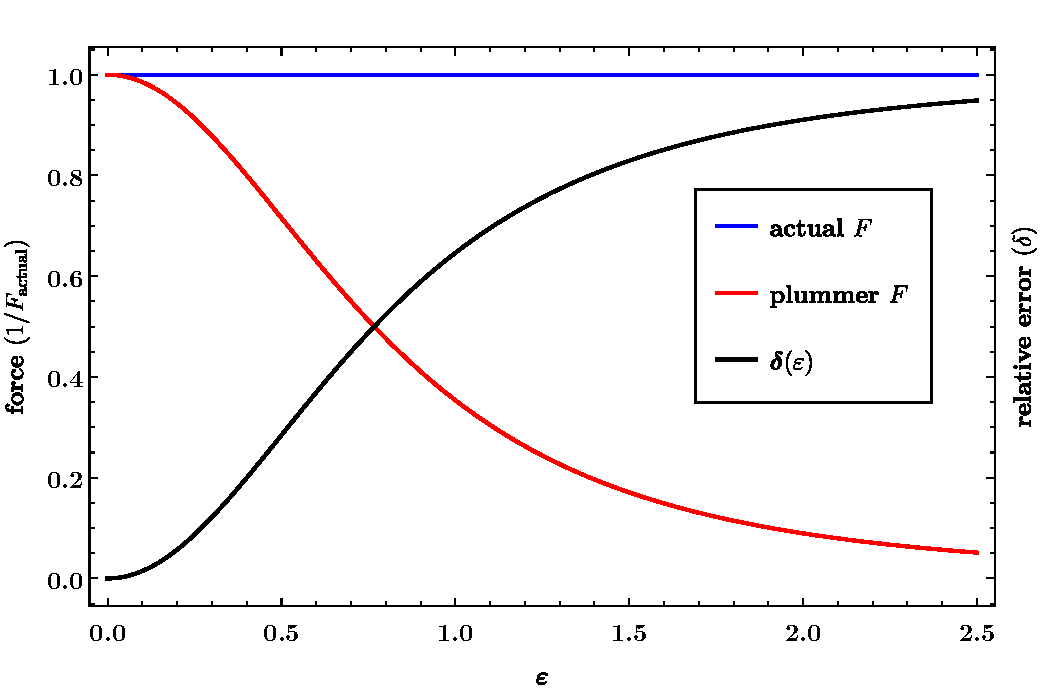
\includegraphics[width=.9\textwidth]{errorepsilon.pdf}}
\label{fig:epsilonerrs}
\end{figure}

\subsection{Modelling Collisions} \label{subsec:collision}
In modelling the collisions between two objects, we make use of an impulse based model. That is, when two collisional particles $i$ and $j$ have collided, we compute an impulse on each of the particles $J$ along the collision normal vector $\vu{n}$, which we'll consider to be the collisional normal vector on $i$ from $j$. If we consider the change in the momentum for the two particles, we can set up a simple system
\begin{subequations} \label{eq:deltmom}
	\begin{align}
		& \Delta \va{P}_i = m_i\va{v}_i^\prime - m_i\va{v}_i \label{eq:momi} \\
		& \Delta \va{P}_j = m_j\va{v}_j^\prime - m_j\va{v}_j \label{eq:momj}
	\end{align}
\end{subequations}

\noindent Given that $J$ is going to conserve the momentum of the particles, we can modify \eqref{eq:deltmom} to yield
\begin{subequations} \label{eq:impulsemom}
	\begin{align}
		 J \vu{n} & = m_i\va{v}_i^\prime - m_i\va{v}_i \label{eq:impulsei}  \\
		-J \vu{n} & = m_j\va{v}_j^\prime - m_j\va{v}_j \label{eq:impulsej}
	\end{align}
\end{subequations}

\noindent or, rearranging and solving for $\va{v}_i^\prime$ and $\va{v}_j^\prime$
\begin{subequations} \label{eq:newvels}
	\begin{align}
		 \va{v}_i^\prime = \va{v}_i + \dfrac{J \vu{n}}{m_i} \label{eq:newvi} \\
		 \va{v}_j^\prime = \va{v}_j - \dfrac{J \vu{n}}{m_j} \label{eq:newvj}
	\end{align}
\end{subequations}

Assuming a perfectly elastic collision (that is, one with a coefficient of restitution $\epsilon = 1$), we can produce the equation
\begin{equation} \label{eq:newoldvrel}
\va{v}_{\text{rel}}^\prime \cdot \vu{n} = -\va{v}_{\text{rel}} \cdot \vu{n} 
\end{equation}

\noindent where $\va{v}_{\text{rel}}^\prime$ and $\va{v}_{\text{rel}}$ is the relative velocity vector between $i$ and $j$ from $i$ after and before the collision, respectively. The expression $\va{v}_{\text{rel}}^\prime \cdot \vu{n}$ may also be expressed by
\begin{equation} \label{eq:vreldiff}
\va{v}_{\text{rel}}^\prime \cdot \vu{n} = (\va{v}_i^\prime - \va{v}_j^\prime) \cdot \vu{n}
\end{equation}

\noindent Substituting in the values for $\va{v}_i^\prime$ and $\va{v}_j^\prime$ from \eqref{eq:newvels} and expressing $\va{v}_{\text{rel}}^\prime$ in terms of $\va{v}_{\text{rel}}$ from \eqref{eq:newoldvrel} and simplifying produces
\begin{equation}
-\va{v}_{\text{rel}} \cdot \vu{n} = \va{v}_{\text{rel}} \cdot \vu{n} + J\vu{n}(\dfrac{1}{m_i} + \dfrac{1}{m_j}) \cdot \vu{n}
\end{equation}
along with multiple regions
\noindent and solving for our impulse
\begin{equation} \label{eq:impulse}
J = -2 \dfrac{\va{v}_{\text{rel}} \cdot \vu{n}}{\frac{1}{m_i}+\frac{1}{m_j}}
\end{equation}

\noindent This equation for our impulse magnitude we can now finally use to derive new velocity vectors for $i$ and $j$ using the formulas we set up in \eqref{eq:impulsemom}
\begin{subequations} \label{eq:newvs}
	\begin{align}
		\va{v}_i^\prime & = -2 \dfrac{(\va{v}_i-\va{v}_j)}{1+\frac{m_i}{m_j}} + \va{v}_i \\
		\va{v}_j^\prime & =  2 \dfrac{(\va{v}_i-\va{v}_j)}{1+\frac{m_j}{m_i}} + \va{v}_j
	\end{align}
\end{subequations}

\noindent Notice that the collision normal vector $\vu{n}$ is not present in our final equation. The final order of business is to tackle when collisions themselves happen. For that we use the same octree that we describe in \ref{subsec:bh}. We search up the tree starting from a given particle and search up the tree a number of layers $n$, and if the criterion $r < \varepsilon$ is satisfied---where $r$ is the distance between two particles in the neighboring nodes and $\varepsilon$ is the plummer softening parameter from \ref{subsec:gravity}---we compute the new collision velocities and run a single timestep to update their position until they are no longer colliding with any particles.

\section{Force Calculation} \label{sec:force}
\subsection{Direct Method} \label{subsec:dm}
With the general form for the magnitude of forces between two particle pairs, we can apply a force vector $\va{F}_{ji}$ to $i$, that is the force vector on $i$ from $j$, by multiplying our force magnitude by the normal vector which points from $i$ to $j$
\begin{equation}
\va{F}_{ji} = G r_{ji} \dfrac{m_im_j}{(r_{ji}^2 + \varepsilon^2)^\frac{3}{2}} \dfrac{\va{r}_j - \va{r}_i}{|\va{r}_j - \va{r}_i|}
\end{equation}

\noindent where $\va{r}_j$ and $\va{r}_i$ are the position vectors of $j$ and $i$ respectively. Applying this same step to \eqref{eq:newtongrav} and noting that $r_{ji} = |\va{r}_j-\va{r}_i|$, we can produce the following softened and unsoftened force equations:
\begin{subequations} \label{eq:\theequation}
	\begin{align}
		& \va{F}_{ji} = G \dfrac{m_im_j}{(r_{ji}^2 + \varepsilon^2)^\frac{3}{2}} ({\va{r}_j - \va{r}_i}) \label{eq:fplum} \\[10pt]
		& \va{F}_{ji} = G \dfrac{m_im_j}{r_{ji}^3}(\va{r}_j-\va{r}_i) \label{eq:fnorm}
	\end{align}

\end{subequations}

Now that we have formulae for computing the force vector applied to $i$ from $j$, we can use Newton's second law to derive the acceleration vector $\va{a}_i$
\begin{equation} \label{eq:\theequation}
\va{a}_i = \dfrac{\sum_{j \neq i}^N \limits \va{F}_{ji}}{m_i}
\end{equation}

\noindent Inserting in \eqref{eq:fplum} and \eqref{eq:fnorm} yields the following set of equations
\begin{subequations} \label{eq:\theequation}
    \begin{align}
		& \va{a}_i = \sum_{j \neq i}^{N} G \dfrac{m_j}{(r_{ji}^2 + \varepsilon^2)^\frac{3}{2}} (\va{r}_j - \va{r}_i) \label{eq:aplum} \\
		& \va{a}_i = \sum_{j \neq i}^{N} G \dfrac{m_j}{r_{ji}^3} (\va{r}_j - \va{r}_i) \label{eq:anorm}
    \end{align}
\end{subequations}

\noindent where \eqref{eq:anorm} provides an exact $\va{a}_i$ and \eqref{eq:aplum} a softened one. These two equations are the backbone of the direct method implementation in SINGS, which we also use as a reference to compare the force calculations provided by other methods, particularly Equation \eqref{eq:aplum} as it exactly gives particle accelerations. The chief drawback of the direct method is that computations scale in order $\mathcal{O}(N^2)$, which for simulations with large $N$ necessitates the use of other force codes.

\subsection{Barnes-Hut} \label{subsec:bh}
The algorithm described by \citet{barnes1986hierarchical} (hereafter Barnes-Hut) is a hierarchical tree algorithm that scales with order $\mathcal{O}(N\log N)$. The Barnes-Hut tree is constructed by recursively partitioning the simulation space into a sequence of cubes, with each cube containing 8 child cubes representing an octant of the parent cube. These cubes form an octree structure, where each cube is a node in the octree. We construct the octree starting with one node representing the whole simulation space, and then partition it in such a way that each node either 0 or 1 particle, or is itself a parent to more nodes. We call nodes of the first variety external nodes, and the second internal nodes. The internal nodes store the center of mass and total mass information of all their internal particles, such that they can be used for approximate force calculation. A diagram illustrating the construction of a Barnes-Hut tree is shown in Figure \ref{fig:bhtree}.

\begin{figure}[h] 
\caption{An illustration of a 2 dimensional Barnes-Hut tree down to various depths $n$. From the base layer, the space is subdivided until all particles occupy external nodes.}
\centerline{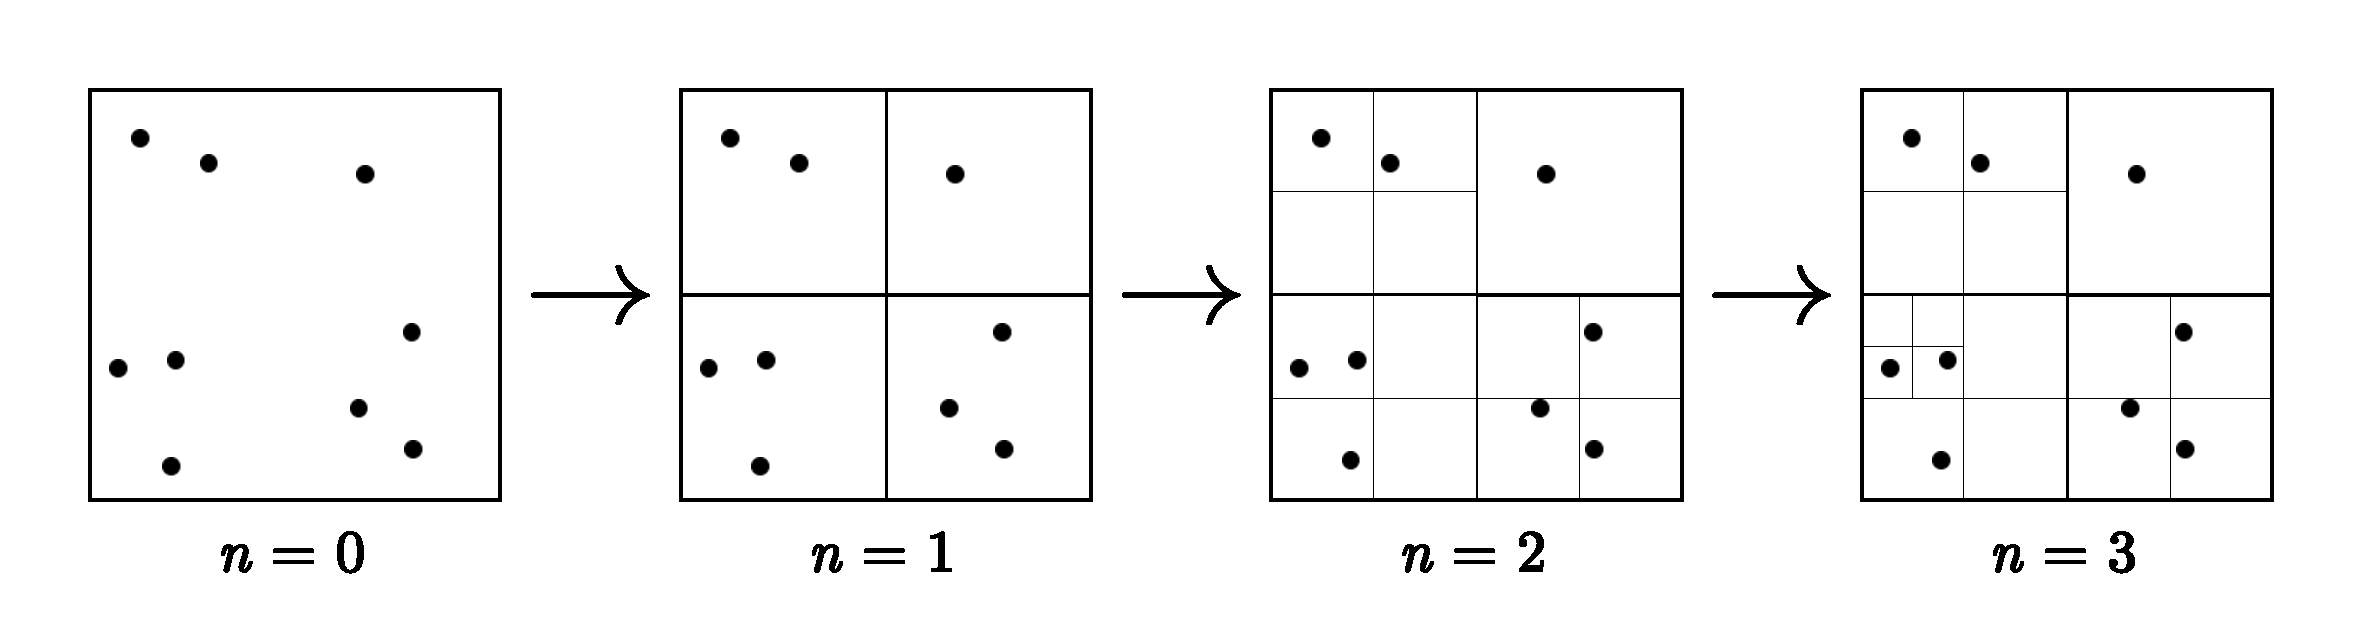
\includegraphics[width=\textwidth]{bhconstruction.pdf}}
\label{fig:bhtree}
\end{figure} 

We then calculate the force on a particle by walking the tree and summing all the approximate forces. In traversing the tree, we  approximate a node as a particle if the relation
\begin{equation} \label{eq:bhcriteria}
\frac{l}{r} < \, \theta
\end{equation}

\noindent is met, where $l$ is the length of the node, $r$ is the distance from the particle to the node, and $\theta$ is a tuneable accuracy parameter. If a node doesn't satisfy \eqref{eq:bhcriteria}, we expand the node, testing on its child nodes. If we end up on an external node with a particle we do a direct particle-particle force calculation before traversing back up through the tree. These steps are repeated until all internal nodes satisfying \eqref{eq:bhcriteria} and other external nodes are visited.

Larger values of $\theta$ will result in larger approximations and thus larger errors, but will also result in reduced compute times. As $\theta \rightarrow 0$, computations tend to grow with order $\mathcal{O}(N^2)$, and the computations become exactly those of the direct method at $\theta = 0$.  The force calculation errors of Barnes-Hut for various values of $\theta$ is shown in Figure \ref{fig:errortheta}.
as computed across various SINGS simulations.
\begin{figure}[h]
\caption{The average error in computed forces for various $\theta$ compared against the direct method across 100 sims/$\theta$, given by $\textbf{error}(\theta) = \dfrac{|\va{F}_{\text{BH}(\theta)}-\va{F}_{\text{Direct}}|}{|\va{F}_{\text{Direct}}|}$.}
\centerline{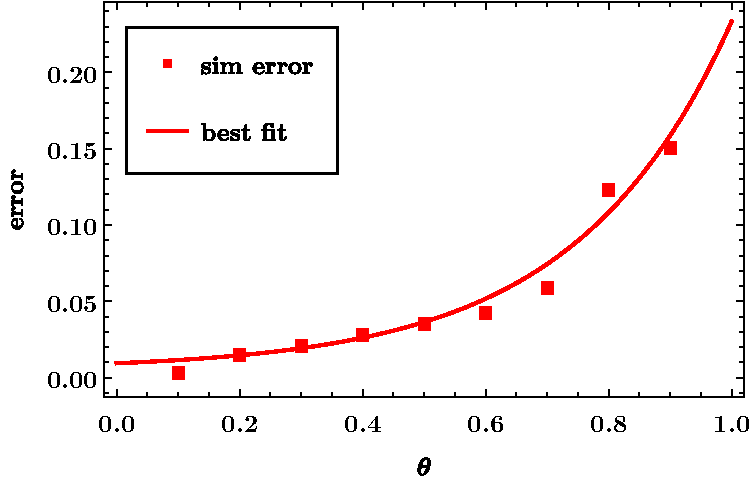
\includegraphics[width=.7\textwidth]{errortheta.pdf}}
\label{fig:errortheta}
\end{figure}

These errors though are more than manageable for carefully chosen values of $\theta$, and allow us to simulate far larger and more complex systems. Figure \ref{fig:sings1bh} features frames from the 2 dimensional SINGS 1 code illustrating the massive reduction in computations enabled by the Barnes-Hut method.
\begin{figure}
\centering
\setlength{\fboxsep}{-1pt}
\setlength{\fboxrule}{1pt}
\begin{subfigure}[t]{.45\textwidth}
  \centering
  \fbox{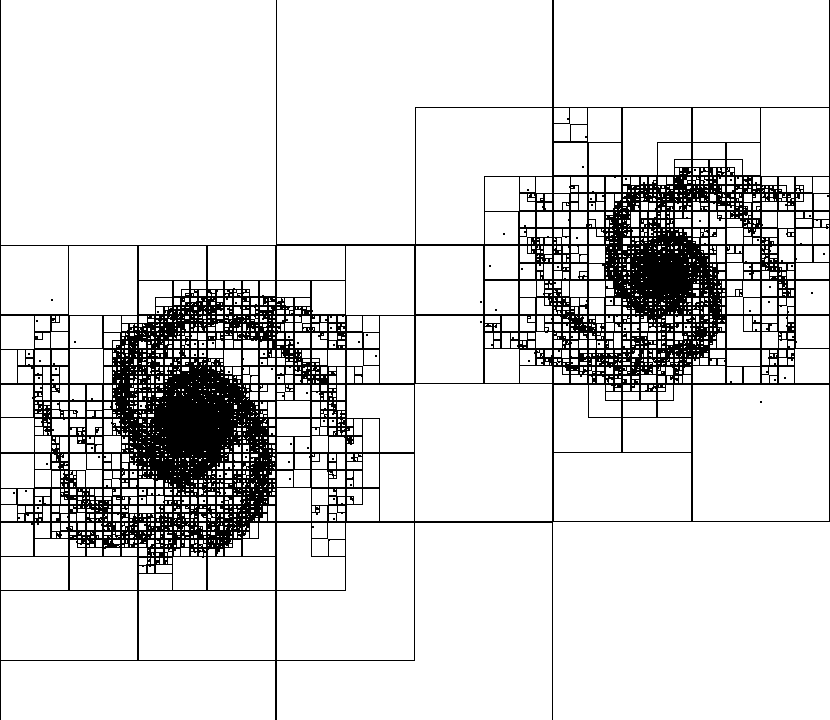
\includegraphics[width=.9\textwidth]{sings1fulltree.png}}
  \label{fig:sub1}
\end{subfigure}%
\begin{subfigure}[t]{.45\textwidth}
  \centering
  \fbox{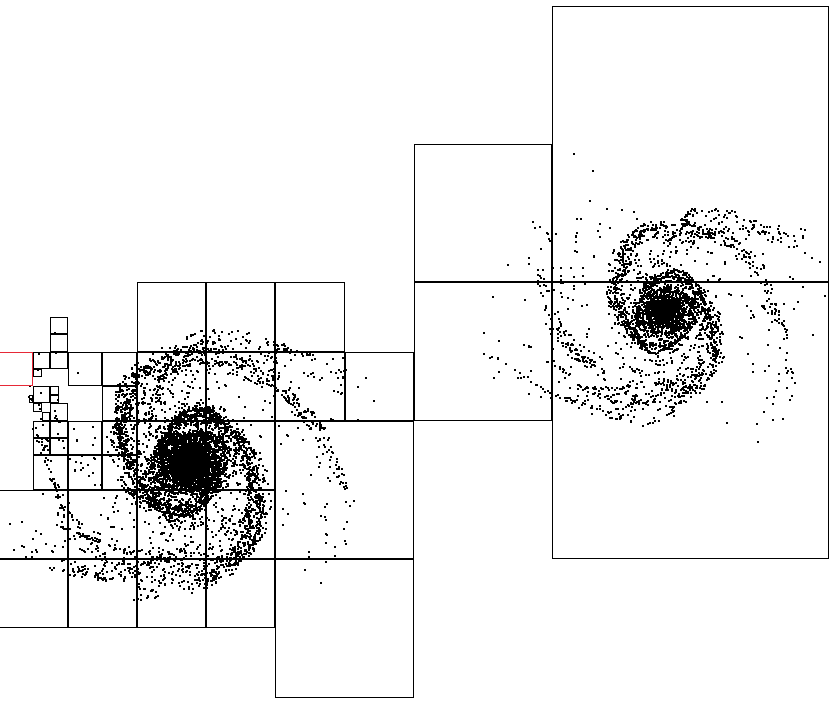
\includegraphics[width=.9\textwidth]{sings1sometree.png}}
  \label{fig:sub2}
\end{subfigure}
\caption{A 2 dimensional SINGS 1 simulation of 12,000 particles, modelling the collision between two galaxies. The frame on the left features the Barnes-Hut tree, the one on the right, the nodes used in calculating the force on a particle on the far left.}
\label{fig:sings1bh}
\end{figure}


\section{Integration} \label{sec:integration}
In this section, we discuss various methods of numerical integration for updating particle positions and velocities given the acceleration vectors generated by our force codes we describe in Section \ref{sec:force}. Two of the methods we describe are energy-conserving under Hamiltonian mechanics, that is, they are symplectic integrators. The others are general integration schemes which can still maintain high order accuracy for certain choices of timesteps $\Delta t$. Regarding timesteps, we use a static timestep as opposed to adaptive, particle-specific timesteps for the purpose of simplicity. Adaptive timesteps allow various particles to take on lower or higher accuracy timesteps appropriately, which generally results in higher accuracy simulations \citep{aarseth1963dynamical}. However, the complexity they introduce resulted in us sticking to fixed particle time steps.

\subsection{Euler Methods} \label{subsec:euler}
The two Euler methods are the simplest methods we include in SINGS for the purpose of numerical integration. We include a second order version of the standard Euler method, where new velocities and positions are derived from
\begin{subequations} \label{eq:euler}
	\begin{align}
		\va{r}_{i+1} & = \va{r}_i + \va{v}_i \Delta t \\
		\va{v}_{i+1} & = \va{v}_i + \va{a}_i \Delta t
	\end{align}
\end{subequations}

\noindent where $\va{r}_{i}$, $\va{v}_i$, and $\va{a}_i$ are the position, velocity, and acceleration vectors of a particle at a timestep $i$ respectively. This method is non-symplectic and has first order error. Given the low order of the error and its non-symplectic nature, this is generally not recommmended as an integrator except for stable simulation configurations (such as modelling planetary orbits.)

The other Euler method SINGS employs is the symplectic (sometimes, the semi-implicit) Euler method, which computes the updated position vector using the new velocity vector as such
\begin{subequations} \label{eq:seuler}
	\begin{align}
		\va{v}_{i+1} & = \va{v}_i + \va{a}_i \Delta t \\
		\va{r}_{i+1} & = \va{r}_i + \va{v}_{i+1} \Delta t
	\end{align}
\end{subequations}
\noindent Note that the order in which these computations have been made is flipped from \eqref{eq:euler}. While this method is still of the first order, its symplectic nature makes it ideal for simple and even relatively complex simulations.

\subsection{Runge-Kutta} \label{subsec:rk4}
The Runge-Kutta method is a non-symplectic method in SINGS. It computes functional derivatives at times between $t$ and $t + \Delta t$, and weights them to produce a prediction for the function at the next time step. The method we use, the fourth-order Runge-Kutta method (henceforth RK4) has fourth order error, which makes it quite appealing despite it's non-symplectic nature.

If we consider $\va{y}_i$ to be a vector containing the dependent variables of our system $\langle \va{r}_i, \va{v}_i \rangle$ and $\va{f}$ to be a vector containing the derivatives of $\va{y}_i$, we can compute $\va{y}_{i+1}$ for our second order system by 
\begin{subequations} \label{eq:rk4}
	\begin{align}
		k_1 & = \Delta t \, \va{f}(t, \va{y}_i)\\
		k_2 & = \Delta t \, \va{f}(t + \frac{1}{2} \Delta t, \va{y}_i + \frac{1}{2} k_1) \\
		k_3 & = \Delta t \, \va{f}(t + \frac{1}{2} \Delta t, \va{y}_i + \frac{1}{2} k_2) \\
		k_4 & = \Delta t \, \va{f}(t + \Delta t, \va{y}_i + k_3) \\
		\va{y}_{i+1} & = \frac{1}{6}(k_1 + 2k_2 + 2k_3 + k_4)
	\end{align}
\end{subequations}

\noindent where $k_1$, $k_2$, $k_3$, and $k_4$ are the RK4 weights. In order to compute the various values of $\va{f}$, we propagate each individual the particle forward at their old velocity $\va{v}_i$ at the timesteps which are specified by the RK4 coefficeints. So while the integrator itself remains $\mathcal{O}(N)$ like all the other integrators, we are having to calculate the force on each particle at those new locations 4 separate times, thus compared to other integrators we'd expect to see compute times at least 4 times greater.

\subsection{Leapfrog Integration} \label{subsec:leapfrog}
Leapfrog integration is the final integration method provided by SINGS, and is the primary one used in major astrophysical simulation tools like GADGET (\citet{springel2005simulating}, \citet{springel2021simulating}). The Leapfrog integrator is a 3rd order symplectic integrator, where with our fixed timesteps we calculate our position and velocity vectors by
\begin{subequations} \label{eq:leapfrog}
	\begin{align}
		\va{r}_{i+1} & = \va{r}_i + \va{v}_i \Delta t + \va{a}_i \Delta t^2 \\
		\va{v}_{i+1} & = \va{v}_i + \frac{1}{2}(\va{a}_{i+1} + \va{a}_i) \Delta t
	\end{align}		
\end{subequations}

This simple scheme allows us to quickly integrate our simulation in a similar time to the Euler methods, yet with significantly lower computational error provided by the Leapfrog integrator's 3rd order accuracy.

\section{Computation} \label{sec:CS}
Here we detail the specific programming aspects of SINGS, discussing the architecture of the program, the libraries we used, and specific challenges during development.

\subsection{Why C?} \label{subsec:vanillac}
SINGS is programmed entirely in vanilla C using the C99 standard for the Linux kernel. No external libraries were used with the exception of OpenMP, which we discuss further in \ref{subsec:parallelisation}. The reason we chose C to write SINGS was its simplicity and performance. The object oriented features of other languages like C++ wouldn't be particularly useful and we felt would only result in code ambiguity. C provided a simple framework where major program elements, like the simulation state, particles, and the functions which act on them, boiled down to passing structs between functions. That simplicity, coupled with the far higher performance from C being a low-overhead, compiled language made it ideal for the high computational demands of SINGS. 

\subsection{Modularity} \label{subsec:modularity}
The basic architecture of SINGS is highly modular, with SINGS execution split into 5 primary steps, those being:
\begin{enumerate}
	\item Simulation Initialisation
	\item Force Calculation
	\item Particle Integration
	\item Collision Resolution
	\item Simulation Serialisation
\end{enumerate}

In the first step, SINGS reads in a snapshot and parameterfile. The latter of which is used to build the internal simulation structure, and the former sets the internal simulation variables that'll be used. During the force calculation stage, the specified force code is applied to all the particles in the simulation, and when completed, pass the particles off to the desired integrator to have their positions updated. Before we pass off the simulation to be serialised, we resolve any particle collisions via the methods outlined in \ref{subsec:collision}. In the last step, the simulation may be serialised and saved into a snapshot file. This doesn't necessarily mean the simulation has concluded, but rather that by user specification in the parameterfile---specifically snapshot frequency---that the current timestep is one that we output. Large simulations have snapshots that may take up many gigabytes, and so allowing the user to choose the rate at which we write those snapshots to the disk paramount, lest we run the risk of losing a run because of a crash, or filling up the disk if we were to serialise every frame. Finally. Assuming the simulation still isn't complete, we revert back to step 2 and propagate the simulation forwards. A graphical representation of this entire process is shown in Figure \ref{fig:modular}.
\begin{figure}
\caption{A flowchart illustrating the large scale architecture of SINGS, in particular the standard runtime loop between the 5 main execution stages.}
\centerline{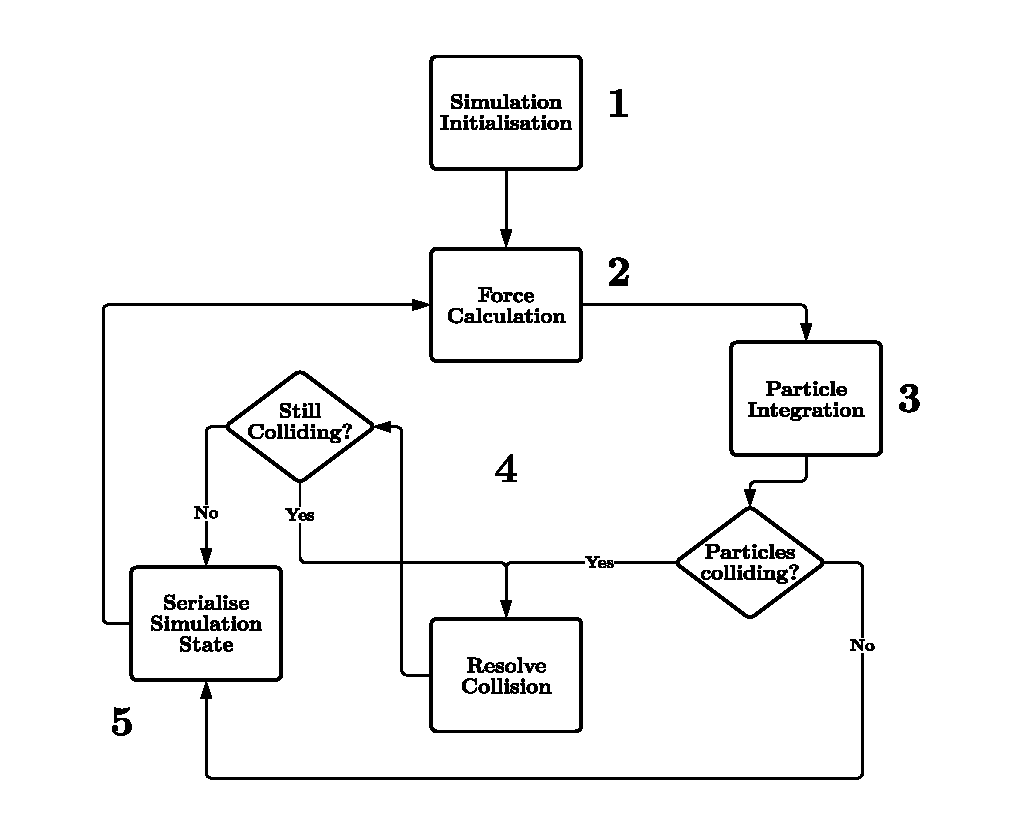
\includegraphics[width=.8\textwidth]{Flowchart.pdf}}
\label{fig:modular}
\end{figure}

A significant advantage in segmenting SINGS execution into these 5 stages is that they each remain completely compartmentalised. No modification to any one of the discrete parts of SINGS requires modification of any of the others.

To illustrate this point, we'll show the modularity of the code in terms of integrators and force codes (stages 2 and 3) for a single frame of a hypothetical simulation using a leapfrog integration scheme and the direct method.

Here is the main simulation loop, as we are concerned with the integration step, we only include it here. SINGS picks the configured integrator from a list of function pointers called \verb+integrators[]+, and then passes in the simulation and force code from the array of function pointers \verb+force_codes[]+ to run. Given we are using leapfrog integration and the direct method, the indices for \verb+integrators[]+ and \verb+force_codes[]+ and are 3 and 0, respectively.



\scriptsize
\begin{minipage}{\linewidth}
\begin{lstlisting}[language=C, label={lst:main}, frame=single]

//main.c
...
for(int i = 0; i < sim.sim_cfg.timesteps; i++ {
	...
	integrators[sim.sim_cfg.integrator](&sim, force_codes[sim.sim_cfg.force_method]);
	...	
}
\end{lstlisting}
\end{minipage}

\normalsize
For the leapfrog integrator, we must hold on to all of our current particle acceleration vectors so we can complete the integration step \eqref{eq:leapfrog}. We then call our force code. Notice, nothing in the leapfrog integrator touches the force codes, they simply pass the simulation state back and forth. We then run a parallel loop to complete the integration step on each of the particles.
\vspace{0.3cm}

\scriptsize
\begin{minipage}{\linewidth}
\begin{lstlisting}[language=C, label={lst:integration}, frame=single]

//integration.c
...
void leapfrog(state *sim, void (*update)(state*)) {
    vec3 *ai = calloc(sim->num_particles, sizeof(vec3));
    for(int i = 0; i < sim->num_particles; i++) {
        ai[i] = sim->particles[i].acc;
    }
    update(sim);

    #pragma omp parallel for
    for(int j = 0; j < sim->num_particles; j++) {
        sim->particles[j].pos = vec_add(sim->particles[j].pos, 
                                vec_add(vec_scale(sim->particles[j].vel,sim->sim_cfg.dt), 
                                vec_scale(ai[j], .5f * sim->sim_cfg.dt*sim->sim_cfg.dt)));
        sim->particles[j].vel = vec_add(sim->particles[j].vel, 
                                vec_scale(vec_add(ai[j], sim->particles[j].acc),
                                 .5f * sim->sim_cfg.dt));
    }

    free(ai);
}
\end{lstlisting}
\end{minipage}

\normalsize
Finally the force calculation step step, just the implementation of the direct method from \eqref{eq:aplum}. We run a parallel for loop across all the particles. The main aspect of these functions to note is that the implementation of these functions do not inherently matter, as long as they all use the same simulation \verb+state+ structure. All we have done in this 3 step process is pass \verb+sim+ around between these various independent functions

\scriptsize
\begin{minipage}{\linewidth}
\begin{lstlisting}[language=C, label={lst:physics}, frame=single]

//physics.c
...
void direct(state *sim) {
    #pragma omp parallel for
    for(int i = 0; i < sim->num_particles; i++) {
        sim->particles[i].acc = (vec3){0,0,0};
        direct_acc(&sim->particles[i], *sim);
    }
}

void direct_acc(particle *p, state sim) {
    for(int j = 0; j < sim.num_particles; j++) {
        if(p == sim.particles+j)
            continue;
        p->acc = vec_add(p->acc, vec_scale(fg_calc(*p, 
        		 sim.particles[j], sim.sim_cfg), 1/p->mass));
    }
}

\end{lstlisting}
\end{minipage}

\normalsize

\subsection{Parallelisation} \label{subsec:parallelisation}
The parallelisation of SINGS is achieved via the use of OpenMP, the only external library used in this project. We chose OpenMP for its simplicity, as it allowed us to focus on developing an initially single core framework that could later be easily adapted for multple cores. At its heart, SINGS is essentially a bunch of nested loops, loops on particles, whether that for calculating forces on those particles or integrating those forces to find their positions and velocities. Because of the modularity of SINGS and the manner in which our simulation data is stored, the \verb+state+ structure, we can easily parallelise the high level loops which update particle parameters. This can be seen first hand in \ref{lst:integration}, where a simple \verb+#pragma omp parallel for+ is all that's needed to parallelise the algorithms.

To demonstrate the effectiveness of this parallelisation, we ran several simulations using the direct method and our two symplectic integrators with various thread counts up to 12, then normalised the y-axis by taking $1/\text{runtime}$ (we take runtime to be roughly $\propto 1/\text{threads}$). The results of this are shown in Figure \ref{fig:runtimethreads}.
\begin{figure}[h]
\caption{A figure showing $1/\text{runtime}$ for various thread counts between the leapfrog and symplectic Euler integration schemes.}
\centerline{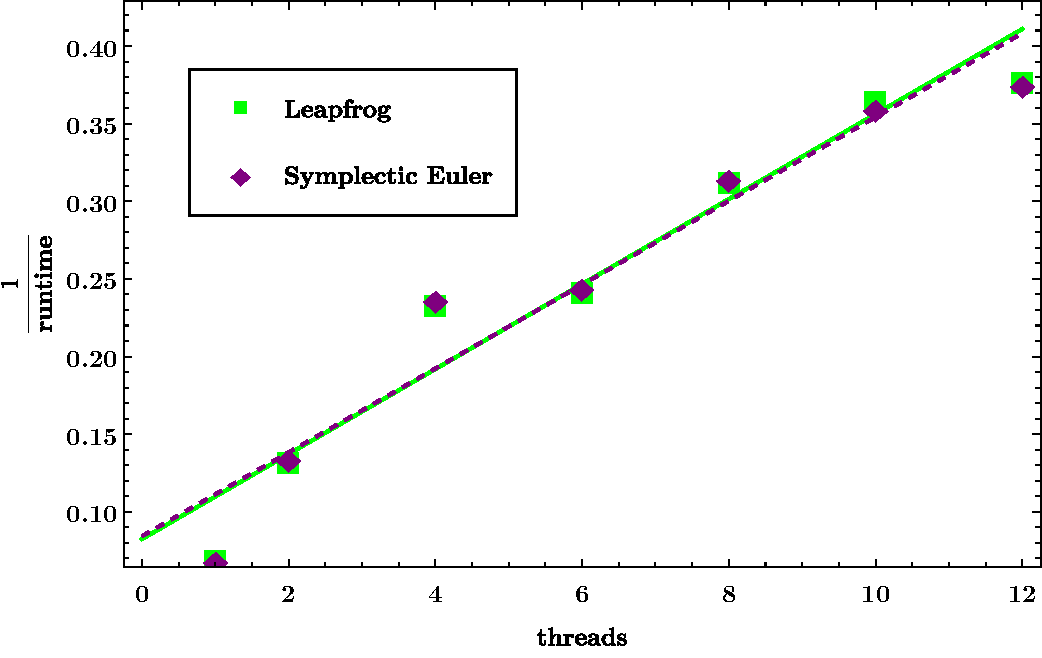
\includegraphics[width=.75\textwidth]{threadsruntime.pdf}}
\label{fig:runtimethreads}
\end{figure}


\subsection{Model Validation} \label{subsec:validation}
We can validate SINGS models by checking for the consistency of certain well known simulation parameters, and seeing how they evolve over the course of a simulation. Examples we've discussed earlier related to Plummer softening \ref{fig:epsilonerrs} and the Barnes-Hut method \ref{fig:errortheta}. Another method besides computing the force directly is measuring the simulation energy. Recalling \ref{subsec:gravity}, 
\begin{equation}
	U = -G \dfrac{m_im_j}{r_{ji}}
	\tag{\ref{eq:newtonpotential}}
\end{equation}

\noindent where $U$ is the gravitational potential energy between two bodies. The only other source of energy in the simulation is going to be the individual particle kinetic energies, given by
\begin{equation} \label{eq:ke}
	K = \frac{1}{2}m_i v_i^2
\end{equation}

\noindent thus, if we want to compute the total mechanical energy $E$ of the simulation at a time $t$, we can do a direct summation over all particle-pairs of their respective gravitational potential energies and ther kinetic energies. Doing this yields
\begin{equation} \label{eq:totenergy}
	E = \sum_{i \neq j}^{N} \frac{1}{2}m_iv_i^2 - G\frac{m_im_j}{r_{ji}}
\end{equation}

This is one of the chief tools SINGS employs for diagnostics, as the reduction or increase in energy of the system over time, while expected (especially with low particle counts with many close-range interactions) might result in unrealistic outputs. A plot featuring the relative energy $E_{\text{rel}}$ (given by $E_{\text{rel}} = \left|\dfrac{E_f - E_i}{E_i}\right|$) across a simulation with various integrators is shown in Figure \ref{fig:energyerror}.
\begin{figure}[h]
\caption{A plot of the relative energy $E_{\text{rel}}$ over the course of a full simulation for various integrator choices.}
\centerline{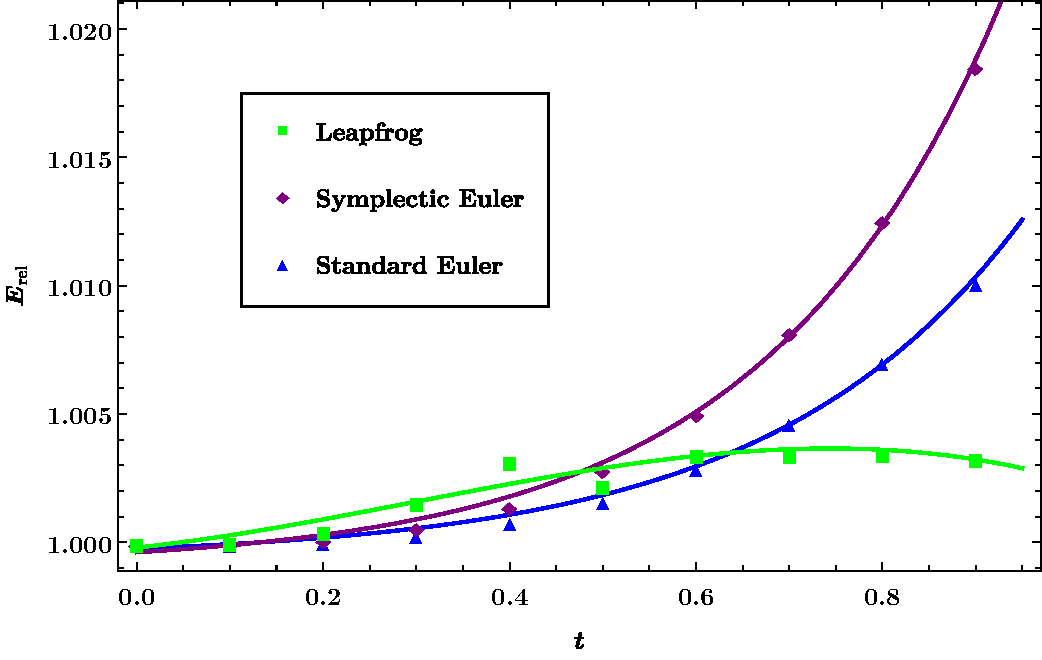
\includegraphics[width=.75\textwidth]{energyerror.pdf}}
\label{fig:energyerror}
\end{figure}

Another measure of error that we haven't yet discussed is the error resulting from high $\Delta t$ values. If we run the same analysis over the course of a simulation, comparing the change in $E_{\text{rel}}$ for various $\Delta t$ we can produce the graph in Figure \ref{fig:energydeltat}.
\begin{figure}[h!]
\caption{The relative change in energy over the course of a simulation using the direct method and different numerical integration methods, for various $\Delta t$ in the range [0, 3.2]}
\centerline{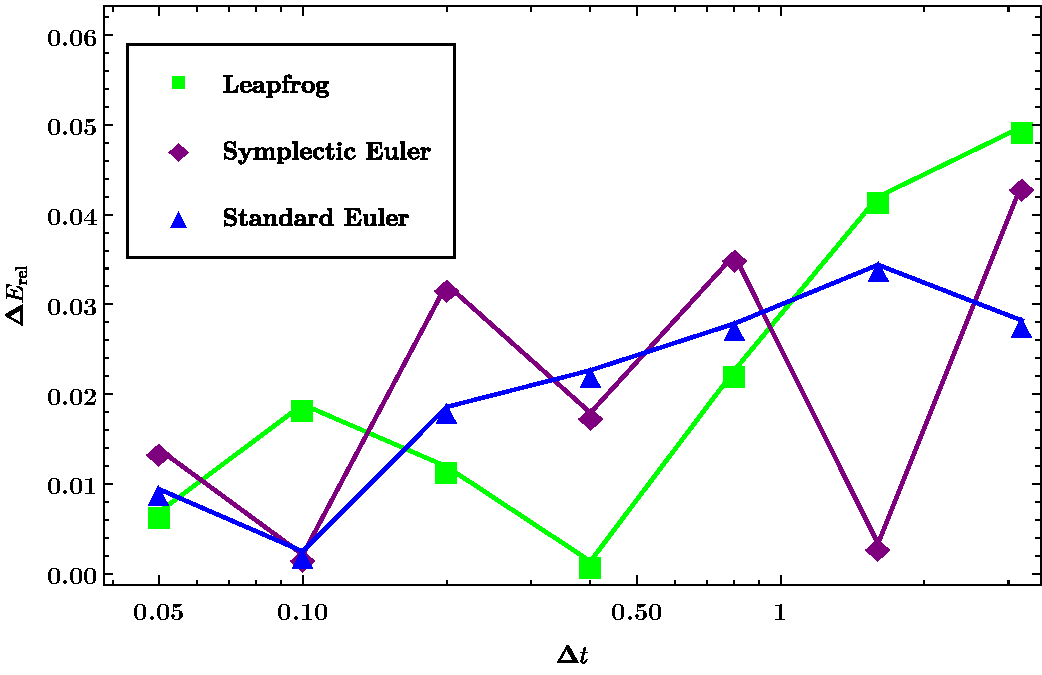
\includegraphics[width=.72\textwidth]{energydeltat.pdf}}
\label{fig:energydeltat}
\end{figure}

We see quite a clean relationship in the change in energy of the system with respect to $\Delta t$ across all integrators, though the randomness of a particular simulation state will mean that at certain $\Delta t$'s deviations from this fit will occur. 

\section{Next Steps} \label{sec:nextsteps}
As powerful a tool as SINGS is today, there are many areas within the codebase that could use improvement along with a plethora of new techniques and approaches to N-body computation which SINGS would benefit immensely from.

A specific example as discussed in the \nameref{sec:abstract} was the Cloud-in-Cell (CIC) Particle Mesh (PM) method. A high level description is that the Particle Mesh method uses a Poison equation and a Fast Fourier Transform (FFT) to compute the gravitational potential in cubic cells across the simulation space. Using this potential we can then apply a  force to a particle inside the cell. This method like Barnes-Hut has an order $\mathcal{O}(N \log N)$, and is particularly well suited for computing the long-range forces on particles extremely quickly (depending on the FFT algorithm), but is less well suited for close interactions. This gives rise to derivations of the method like the Particle-Particle-Particle Mesh (P$^3$M) method \citep{hockney1988particle} which does a direct force calculation between nearby particles. This latter method was initially planned to be in SINGS at release but the present architecture did not adapt well to the method and our FFT was not easily parallelised. However, we feel strongly that the future of SINGS will likely involve some P$^3$M implementation.

A reworking of the architecture to support P$^3$M would also make way for the implementation of a more robust and realistic collisional particle model via Smoothed-Particle Hydrodynamics (SPH) \citep{gingold1977smoothed}. Our current collisional gas model may be accurate if we take the particles to be like individual molecules colliding with one another but in terms of astrophysical simulations, it simply doesn't cut it. In short, SPH is a mesh-free approach to model fluid flows. It approaches the problem by dividing a fluid into discrete moving elements governed by a so-called "kernel function", which mediates particle interactions. The power of SPH as a computationally efficient way to accurately model the fluid-like flows of the interstellar and intergalactic mediums would makes for its would-be implementation in SINGS highly desireable. 

Before tackling any of these problems, however, there exists a major short term goal, and that is the implementation of periodic boundary conditions. These are necessary for high resolution structure formation simulations, and presently SINGS does not support them. In essence, periodic boundary conditions result in particles that leave the simulation space being acted on by mirrors of the simulation space. This is relatively cheap to compute as the force from the mirrors of the simulation can be acquired by a coordinate transformation on the particle. This is a high priority goal, and is likely the first major upgrade to SINGS after the conclusion of the New Mexico Supercomputing Challenge.

A smaller goal is to support a Hubble constant, essentially for modelling cosmic expansion. This would allow SINGS to analyse real $\Lambda$CDM cosmologies, scenarios like those close to the big bang, given the modification to the architecture to handle the numerical errors associated with such extreme conditions. And on the larger scales, it would allow SINGS to analyse structure formation in the context of an expanding universe. This isn't a high priority goal, but compared to some of the other ideas addressed here, it is the one most in reach.

And finally, a distant stretch goal is the implementation of Open MPI. Modifying the architecture to support the segmented memory of supercomputers would allow SINGS to contribute to meaningful research, given the changes we've outlined in this section. The current architecture around OpenMP is exceptionally simple in comparison to what an MPI implementation would take, however, it would truly prove SINGS' worth as a tool for modelling astrophysical systems.

\section{Conclusion} \label{sec:conclusion}
What we have demonstrated through analysis of the data generated by SINGS is that it is an extremely capable tool for running complex astrophysical simulations. While the architecture cannot handle the high particle counts and the collisional dynamics of more mainstream astrophysical simulation codes, it more than holds its own. SINGS thus far has been validated in handling simulations in particle counts in excess of 1,000,000, and with the performance improvements facilitated by the multithreading of OpenMP will surely enable the creation of larger, more complex simulations. OpenMP support brings many opportunities for furthering the development of the software, and its implementation has probably been the single greatest achievement in developing SINGS. The fleshed out Barnes-Hut implementation already provided a strong foundation for further advancements, in addition to SINGS' general architectural modularity. The error diagnostic tools and the simulation i/o, however rudimentary, make SINGS flexible and easy to use for those hoping to make and run astrophysical simulations of their own. With the implementation of certain features discussed in Section \ref{sec:nextsteps}, SINGS has the potential to become far more than just a humble N-body gravitation simulator.

The repositories for SINGS and SINGS I can be found on Github with the following links. Also included is a repository containing all the materials used in the creation of this document, including the raw data files generated from SINGS outputs. SINGS will slowly be released onto the Github under the GPLv2 license, as the source code is polished and documented. However, SINGS I as featured in this paper is already fully available for use, however rudimentary it is in comparison.
\vspace{0.2cm}

\noindent \text{SINGS: }  \href{https://github.com/CodingKraken/SINGS}{\color{blue}{\text{https://github.com/CodingKraken/SINGS}}} 

\noindent \text{SINGS I: } \href{https://github.com/CodingKraken/SINGS-I}{\color{blue}{\text{https://github.com/CodingKraken/SINGS-I}}}

\noindent \text{This Paper and More: } \href{https://github.com/CodingKraken/SCC-SINGS-Paper}{\color{blue}{\text{https://github.com/CodingKraken/SCC-SINGS-Paper}}}

\section*{Acknowledgements} \label{sec:acknowledge}
\addcontentsline{toc}{section}{Acknowledgements}
This project started over 1 year ago as a spring break project. We had just discussed gravitation in AP Physics I, and I was eager to see what I could pull off, while also furthering my familiarity with C. I never could have forseen what this break time project would become.

First off I would also like to thank those involved with the Supercomputing Challenge itself, for putting on such an event to inspire and push people to not only develop their software skills, but also to inspire a love of the art of programming, of STEM subjects in general. I would like to thank Dr. Sharon Deland who provided pointed feedback on my interrim report, and additionally even I only got to know them for half an hour, I would like to thank my February evaluators, Mr. Scott Levy and Mr. Abdalaziz Raad, for taking their time to review my project and my presentation. Their feedback was truly invaluable. I would also like to sincerely thank Karen Glennon, who is providing me the opportunity to go to the expo in person.

And finally, I never would have made it this far were it not for my Project Mentor and Physics teacher of the last two years Dr. Bradley Knockel. He was a constant source of inspiration and insight throughout the entire process, providing ideas, criticism, and motivation, raising concerns of problems I had never even thought to consider, and providing support down avenues of research I could not have approached otherwise. I would not be participating in this competition were it not for his endless support, and for that I am immensely grateful. Additionally, I want to thank my friends who pushed me to continue working on the project, even when I felt there was no moving forward. To all of them I am immensely indebted.

\printbibliography

\end{document}
